\documentclass[a4paper,12pt,oneside]{article} 

\usepackage[utf8]{inputenc}
\usepackage[pdftex]{graphicx}
\usepackage{polski}
\usepackage{amsfonts}
\usepackage{verbatim}
\usepackage{indentfirst}
\usepackage{listings}
\usepackage[polish]{babel}
\usepackage[T1]{fontenc}
\usepackage{fancyhdr}
\usepackage{lastpage}
\pagestyle{fancy}
\renewcommand{\headrulewidth}{0pt}
\rhead{}
\lhead{}
\cfoot{str. \thepage/\pageref{LastPage}}

\begin{document}
\makeatletter
\addtocontents{toc}{\protect\thispagestyle{empty}}
\newcommand{\linia}{\rule{\linewidth}{0.4mm}}

\renewcommand{\maketitle}{\begin{titlepage}

    \vspace*{1cm}

    \begin{center}\small

    Politechnika Warszawska\\

    Wydział Elektryczny\\

    \end{center}

    \vspace*{1cm}

    \noindent\linia

    \begin{center}

      \LARGE \textsc{\@title}

         \end{center}

      \noindent\linia

    \vspace{1cm}

    \begin{flushright}

    \begin{minipage}{5cm}

    \textit{\small Autorzy:}\\

    \normalsize \textsc{\@author} \par

    \end{minipage}
         \end{flushright}
 \begin{center}
    \vspace{5cm}

     {\small Praca wykonana w~ramach przedmiotu:
     Języki i~metody programowania 2}

    \vspace*{\stretch{6}}

    \@date

    \end{center}

  \end{titlepage}

}

\makeatother

\title{Specyfikacja implementacyjna}

\title{SPECYFIKACJA IMPLEMENTACYJNA\\projekt: automat komórkowy}

\author{Anna Głowińska\newline numer indeksu: 291070\newline anna.glowinska98@gmail.com \newline \newline
Adam Czajka\newline numer indeksu: 291063 \newline czajka.adam147@gmail.com}

\maketitle
\tableofcontents
\thispagestyle{fancy}
\newpage

\section{Informacje ogólne}

\subsection{Uruchomienie programu}
Uruchomienie programu \verb+life+ następuje przez wywołanie programu \verb+make+. Po kompilacji i~uruchomieniu program pozwala użytkownikowi wybrać rodzaj sąsiedztwa, liczbę generacji do przeprowadzenia oraz dane wejściowe (generację początkową).
\par Działanie programu \verb+life+ odbywa się w oknie terminala, gdzie przebiega komunikacja między użytkownikiem a programem.


\subsection{Przebieg programu}
Program na podstawie pobranych informacji wykonuje zadaną liczbę generacji. Każdorazowo wypisuje obecną generację na ekran terminala i~oczekuje podania znaku od użytkownika. Po wpisaniu znaku \verb+s+~następuje zapis generacji do pliku PBM, \verb+t+~- zapis generacji do pliku TXT, \verb+q+~- natychmiastowe zakończenie działania progarmu, znaki od \verb+1+~do~\verb+9+~oznaczają przeprowadzenie danej liczby generacji bez zapisywania. Podanie jakiekogolwiek innego znaku jest ignorowane przez program. Wyniki (pliki PBM i~TXT) są zapisywane w~katalogu \verb+life/dane/wyniki+.


\section{Opis modułów}

\subsection{Diagram modułów}

\begin{figure}[ht]
\centering
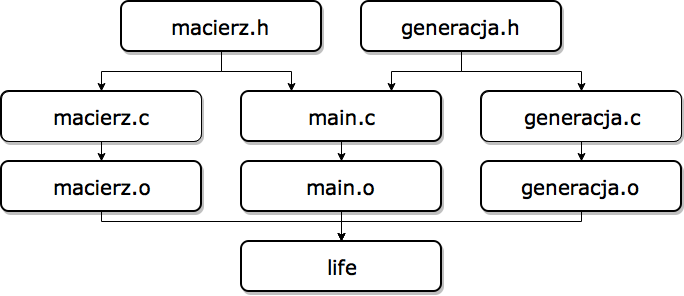
\includegraphics[width=1.0\textwidth]{diagram_modulow.png}
\caption{Diagram modułów.}
\label{fig:k1}
\end{figure}

\subsection{Uzasadnienie}
Diagram modułów programu \verb+life+ ma postać przedstawioną na rysunku nr 1. Moduły są między sobą powiązane relacją zależności, ponieważ wymagają ich do realizacji własnej funkcjonalności. Zależność między dwoma modułami oznaczona jest strzałką i polega na tym, że moduł w stronę którego skierowany jest grot strzałki korzysta drugiego z danych modułów - zmiana w tym module może spowodować konieczność zmiany w module oznaczonym strzałką.

\subsection{Moduł generacja}

\begin{description}
\item[Funkcja \texttt{generuj4()}] \hfill \\
Przeprowadza generację zgodnie z~zasadami ,,Gry w życie'' z~wykorzystaniem sąsiedztwa von~Neumann'a. Po osiągnięciu granicy macierzy układy komórek pojawiają się po przeciwległej stronie kontynuując grę.
\begin{itemize}
\item funkcja jest bezargumentowa,
\item funkcja jest typu \verb+void+ - nie przekazuje informacji zwrotnej.
\end{itemize}
\item [Funkcja \texttt{generuj8()}] \hfill \\
Przeprowadza generację zgodnie z zasadami ,,Gry w życie'' z~wykorzystaniem sąsiedztwa Moore'a. Po osiągnięciu granicy macierzy układy komórek pojawiają się po przeciwległej stronie kontynuując grę.

\begin{itemize}
\item funkcja jest bezargumentowa,
\item funkcja jest typu \verb+void+ - nie przekazuje informacji zwrotnej.
\end{itemize}
\end{description}

\subsection{Moduł macierz}

\begin{description}
\item[Funkcja \texttt{inicjuj()}] \hfill \\
Tworzy dwie macierze (dajej nazywane pierwszą i~drugą macierzą) służące do przechowywania i~przeprowadzania generacji oraz alokuje im miejsce w~pamięci wykorzystując przeczytane z~pliku wejściowego informacje o~wielkości macierzy. Pierwsza macierz zawsze przechowuje obecną generację, a~druga służy do przepisywania danych podczas wykoywania funkcji \verb+generuj4()+ i \verb+generuj8()+.
\begin{itemize}
\item funkcja jako argument przyjmuje wskaźnik do pliku z danymi początkowymi,
\item funkcja jest typu \verb+void+ - nie przekazuje informacji zwrotnej.
\end{itemize}

\item[Funkcja \texttt{wymiary()}] \hfill \\
Zapisuje wymiery \verb+x+~i~\verb+y+~macierzy w adresach podanych przy wywołaniu. Wymiary pierwszej i~drugiej macierzy są takie same.
\begin{itemize}
\item funkcja jako argumenty przyjmuje wskaźniki do dwóch liczb całkowitych, które są szerokością oraz długością macierzy z danymi pierwotnymi,
\item funkcja jest typu \verb+void+ - nie przekazuje informacji zwrotnej.
\end{itemize}

\item[Funkcja \texttt{wstaw()}] \hfill \\
Wstawia wartość \verb+w+~podaną przy wywołaniu w~\verb+x+-owe (również podane przy wywołaniu) miejsce pierwszej macierzy.
\begin{itemize}
\item funkcja jako argumenty przyjmuje dwie liczby całkowite, z których jedna jest indeksem macierzy, gdzie będzie podstawiana druga wartość,
\item funkcja jest typu \verb+void+ - nie przekazuje informacji zwrotnej.
\end{itemize}

\item[Funkcja \texttt{wstaw2()}] \hfill \\
Wstawia wartość \verb+w+~podaną przy wywołaniu w miejsce drugiej macierzy o~współrzędnych \verb+x+~\verb+y+~również podanych przy wywołaniu.
\begin{itemize}
\item funkcja jako argumenty przyjmuje trzy liczby całkowite, z których dwie są współrzędnymi macierzy, gdzie będzie podstawiana trzecia wartość,
\item funkcja jest typu \verb+void+ - nie przekazuje informacji zwrotnej.
\end{itemize}

\item[Funkcja \texttt{wartosc()}] \hfill \\
Zwraca wartość komórki pierwszej macierzy o podanych współrzędnych \verb+x+ \verb+y+.
\begin{itemize}
\item funkcja jako argumenty przyjmuje dwie liczby całkowite, które są współrzędnymi macierzy,
\item funkcja jest typu \verb+int+ - zwraca liczbę całkowitą.
\end{itemize}

\item[Funkcja \texttt{wartosc2()}] \hfill \\
Zwraca wartość \verb+x+-owej komórki drugiej macierzy.
\begin{itemize}
\item funkcja jako argument przyjmuje liczbę całkowitą, która jest indeksem macierzy,
\item funkcja jest typu \verb+int+ - zwraca liczbę całkowitą.
\end{itemize}

\item[Funkcja \texttt{czytaj()}] \hfill \\
Czyta dane z~pliku podanego przy wywołaniu do pierwszej macierzy.
\begin{itemize}
\item funkcja jako argument przyjmuje wskaźnik do pliku z danymi początkowymi,
\item funkcja jest typu \verb+void+ - nie przekazuje informacji zwrotnej.
\end{itemize}

\item[Funkcja \texttt{wypisz()}] \hfill \\
Wypisuje na ekran terminala obecną generację.
\begin{itemize}
\item funkcja jest bezargumentowa,
\item funkcja jest typu \verb+void+ - nie przekazuje informacji zwrotnej.
\end{itemize}

\item[Funkcja \texttt{rysuj()}] \hfill \\
Zapisuje obecną generację do pliku podanego podczas wywołania. Plik jest formatu PBM.
\begin{itemize}
\item funkcja jako argument przyjmuje wskaźnik do pliku z danymi początkowymi,
\item funkcja jest typu \verb+void+ - nie przekazuje informacji zwrotnej.
\end{itemize}


\item[Funkcja \texttt{rysujtxt()}] \hfill \\
Zapisuje obecną generację do pliku podanego podczas wywołania. Plik jest formatu TXT.
\begin{itemize}
\item funkcja jako argument przyjmuje wskaźnik do pliku z danymi początkowymi,
\item funkcja jest typu \verb+void+ - nie przekazuje informacji zwrotnej.
\end{itemize}

\end{description}

\section{Przechowywanie danych}
\subsection{Struktura danych}
Dane wejściowe są zapisywane w~strukturze znajdującej się w~module \verb+macierz+. Struktura zawiera tablicę liczb całkowitych o~wymiarach zgodnych z~danymi wejściowymi oraz dwie liczby całkowite \verb+x+~i~\verb+y+~przechowujące dwa wymiary owej macierzy. 
\par Dostęp do danych znajdujących się w~tej strukturze następuje poprzez wywołanie odpowiednch funkcji modułu \verb+macierz+. Ułatwia to łatwiejsze zlokalizowanie błędnych modyfikacji zawartości tej struktury.

\section{Sprzęt i oprogramowanie}

\subsection{System operacyjny}
Program \verb+life+ jest pisany, kompilowany i~testowany na systemie operacyjnym \verb+macOS High Sierra+. System ten jest z~rodziny \verb+UNIX+.

\subsection{Język programowania}
Program \verb+life+ został napisany w~języku \verb+C+.

\subsubsection{Wersja}
Program został napisany zgodnie ze standardem \verb+ansi+ oraz jest kompilowany przez program \verb+make+ z argumentam \verb+-ansi+.

\subsubsection{Kompilacja}
Do tworzenia pliku wykonywalnego używany jest kompilator \verb+gcc+. Cała procedura nastpuje poprzez wywołanie programu \verb+make+. Przy wywołaniu programu \verb+make+ możliwe są opcje: 
\begin{itemize}
\item uruchomienie programu (podczas którego poszczególne pliki mogą być kompilowane zgodnie z~regułą pliku \verb+Makefile+),
\item sama kompilacja, 
\item \verb+clean+, która powoduje usunięcie wszystkich plików o~rozszerzeniu \verb+o+~z~katalogu \verb+life/src+, plików PBM z~katalogu \verb+life/dane/wyniki+ oraz pliku wykonywalnego \verb+life+ z~katalogu \verb+life/bin+.
\end{itemize}
\par
Kompilacja \verb+gcc+ następuje z argumentami \verb+-pedantic+, \verb+-Wall+ oraz \verb+-ansi+.

\subsection{Testowanie programu}

\subsubsection{Testy}
Do testowania używane są pliki testowe zawierające testy pojedynczych funkcjonalności programu (czytanie z~pliku TXT, czytanie z~pliku PBM, zapisywanie do pliku TXT etc.). Wszystkie pliki zawierające testy przechowywane są w~katalogu \verb+life/src/testy+ i~nazwane zgodnie z~następującą koncepcją: \verb+,,test_co-jest-testowane_co-powinno-być-wynikiem/skutkiem.c''+.

\par
Testy pisane są na zasadzie given-when-then. Oznacza to, że kod każdego testu zostanie podzielony na trzy części:
\begin{itemize}
\item given - odpowiadającą za dane, które test pobiera z~programu,
\item when - wykonująca odpowiednie działania, wywołująca funkcje etc.,
\item then - sprawdzająca poprawność wykonanych działań, wywołanych funkcji etc.
\end{itemize}

\subsubsection{Debugowanie pamięci}
Wycieki pamięci w~programie \verb+life+ są badane i~lokalizowane za pomocą narzędzia \verb+valgrind+.

\section{Wersjonowanie}

\subsection{Branch'e}
Program jest pisany i~commit'owany z~jednej tylko gałęzi \verb+master+, ponieważ w~dwuosobowej zajmującej się tym programem grupie zachowane zostają zasady extreme programming zakładające obecność dwóch osób podczas pisania kodu.

\subsection{Historia wersji}
Historia wersji programu zostaje wypisana na ekran za pomocą komendy \verb+$ git log+. Za pomocą opcji \verb+amend+ można cofnąć zmiany w dowolnym pliku, który był już commit'owany.


\end{document}